\chapter{Extended Access Control
Lists}\label{extended-access-control-lists}

ANOTHER WAY TO CONFIGURE NUMBERED ACLs

\begin{itemize}
\tightlist
\item
  In DAY 34, you learned that numbered ACLs are configured in Global
  Config mode:
\end{itemize}

\begin{figure}
\centering
\pandocbounded{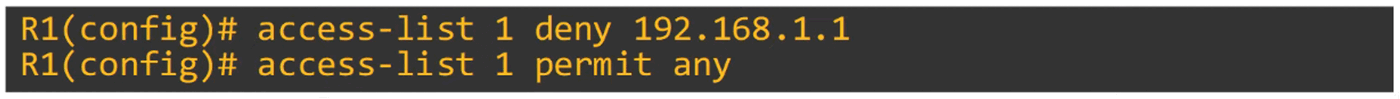
\includegraphics[keepaspectratio,alt={image}]{images/36-extended-access-control-lists/img-001.png}}
\end{figure}

\begin{itemize}
\tightlist
\item
  You learned that named ACLs are configured with subcommands in a
  separate config mode:
\end{itemize}

\begin{figure}
\centering
\pandocbounded{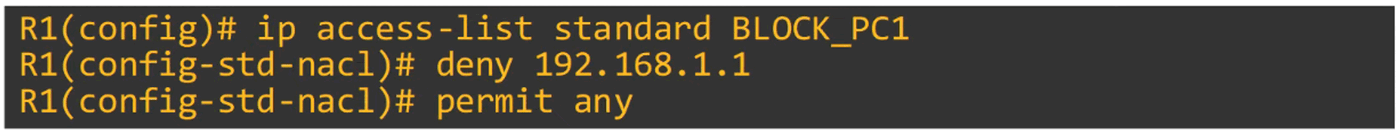
\includegraphics[keepaspectratio,alt={image}]{images/36-extended-access-control-lists/img-002.png}}
\end{figure}

\begin{itemize}
\tightlist
\item
  However, in modern IOS you can also configure numbered ACLs in the
  exact same way as named ACLs:
\end{itemize}

\begin{figure}
\centering
\pandocbounded{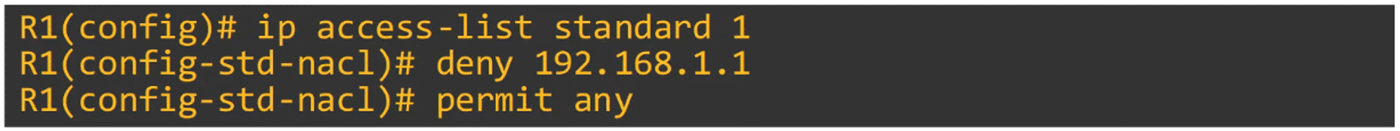
\includegraphics[keepaspectratio,alt={image}]{images/36-extended-access-control-lists/img-003.png}}
\end{figure}

\begin{figure}
\centering
\pandocbounded{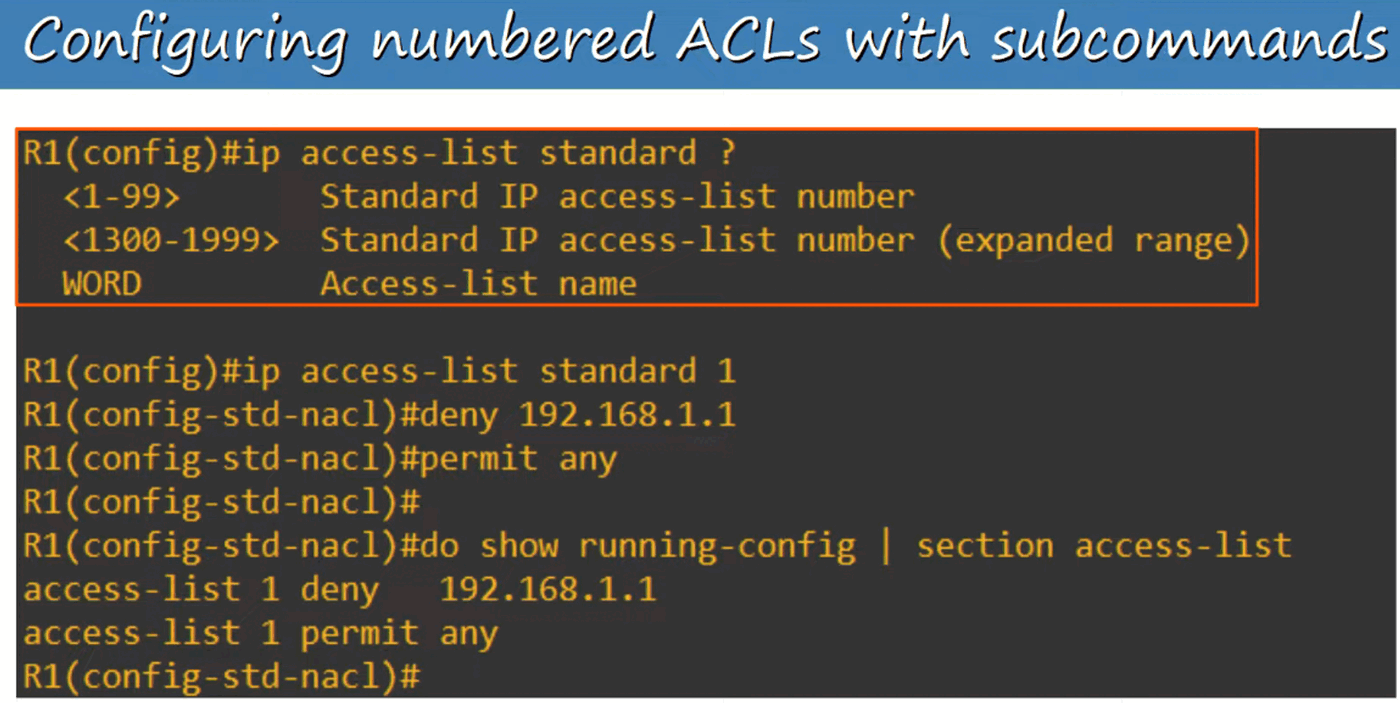
\includegraphics[keepaspectratio,alt={image}]{images/36-extended-access-control-lists/img-004.png}}
\end{figure}

\section{Advantages of Named ACL Config
Mode}\label{advantages-of-named-acl-config-mode}

\begin{itemize}
\tightlist
\item
  You can easily DELETE individual entries in the ACL with NO
  \emph{entry-number}
\item
  You can easily DELETE individual entries in the ACL with NO
  \emph{sequence-number}
\end{itemize}

\begin{figure}
\centering
\pandocbounded{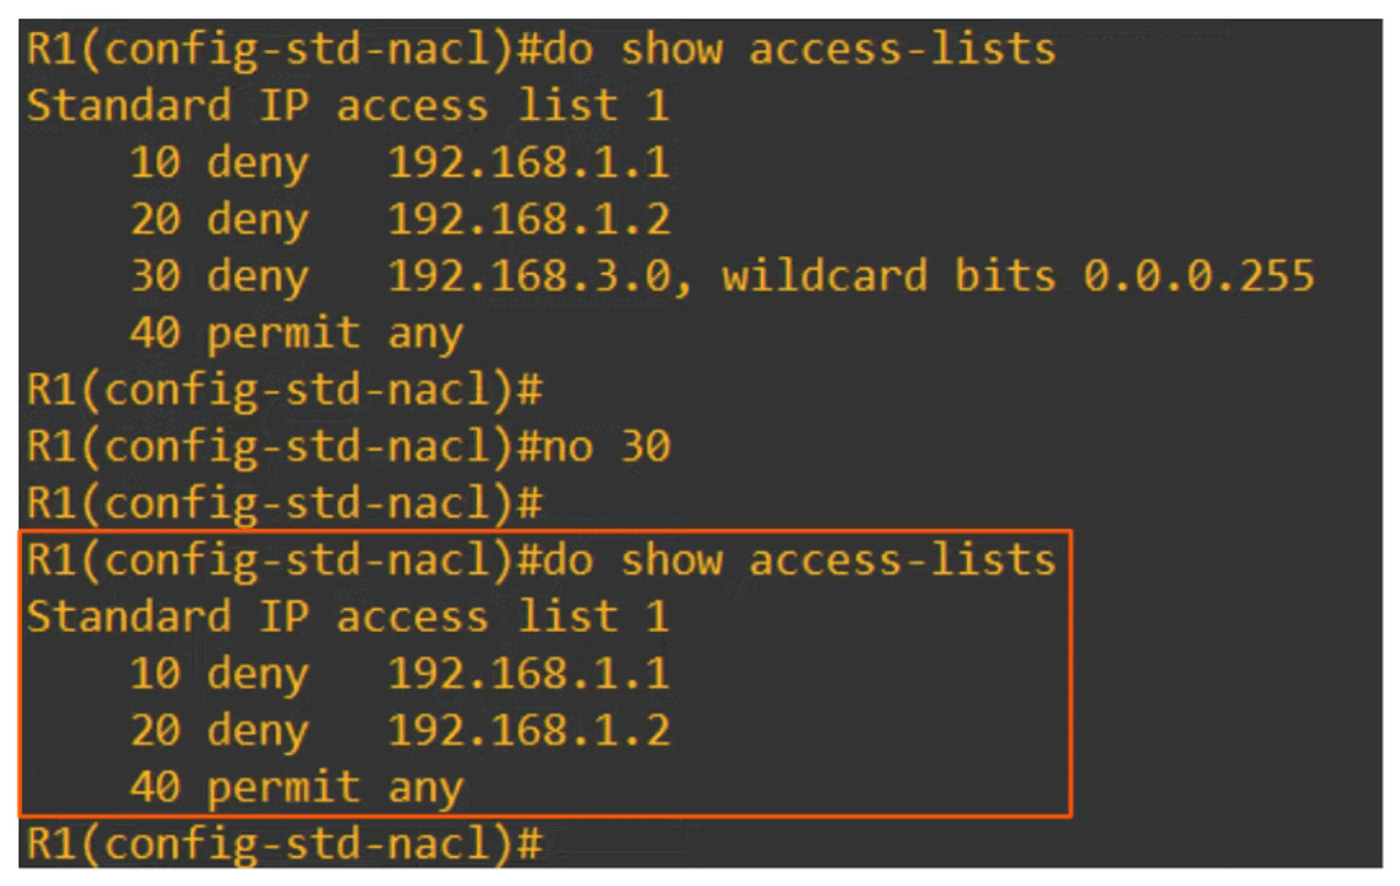
\includegraphics[keepaspectratio,alt={image}]{images/36-extended-access-control-lists/img-005.png}}
\end{figure}

This doesn't work with NUMBERED access lists

\begin{figure}
\centering
\pandocbounded{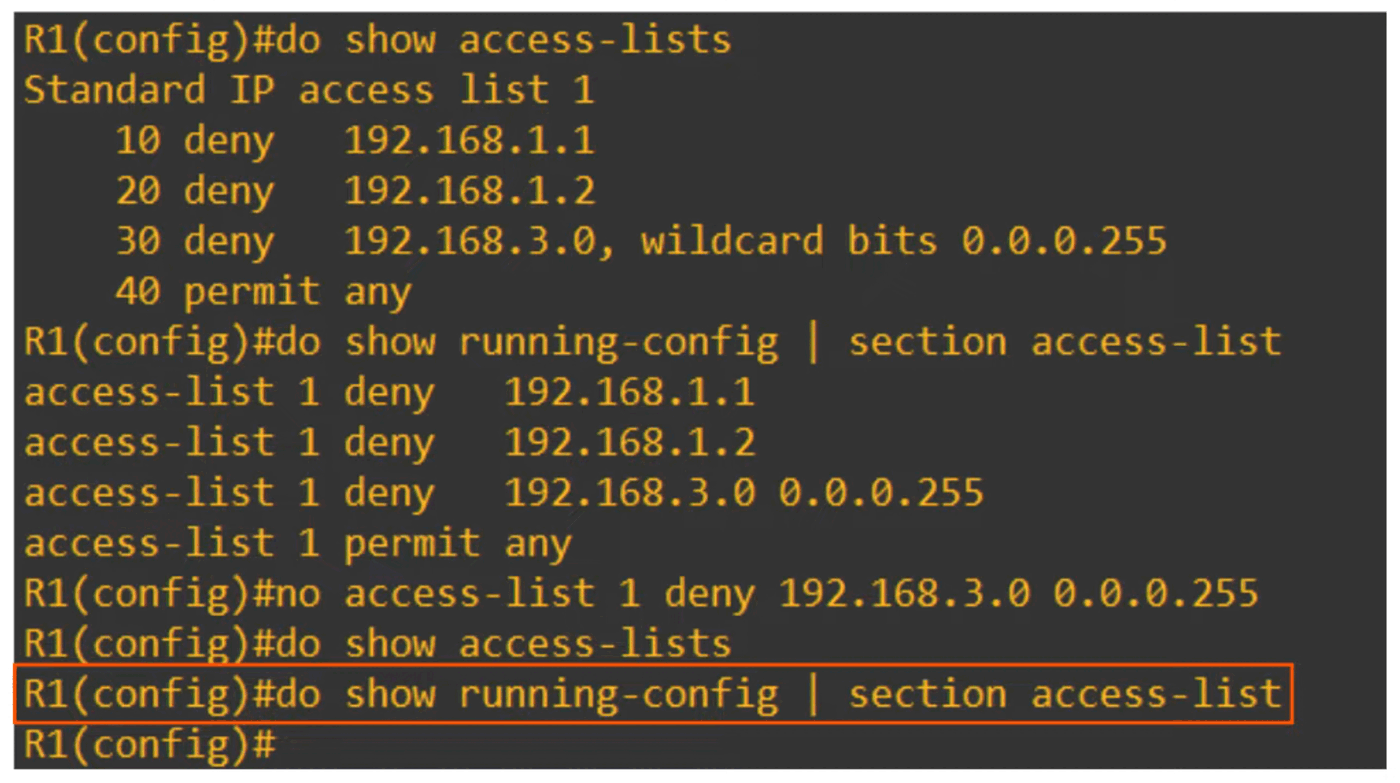
\includegraphics[keepaspectratio,alt={image}]{images/36-extended-access-control-lists/img-006.png}}
\end{figure}

\begin{itemize}
\tightlist
\item
  You can insert NEW entries in-between other entries by specifying the
  SEQUENCE NUMBER
\end{itemize}

\begin{figure}
\centering
\pandocbounded{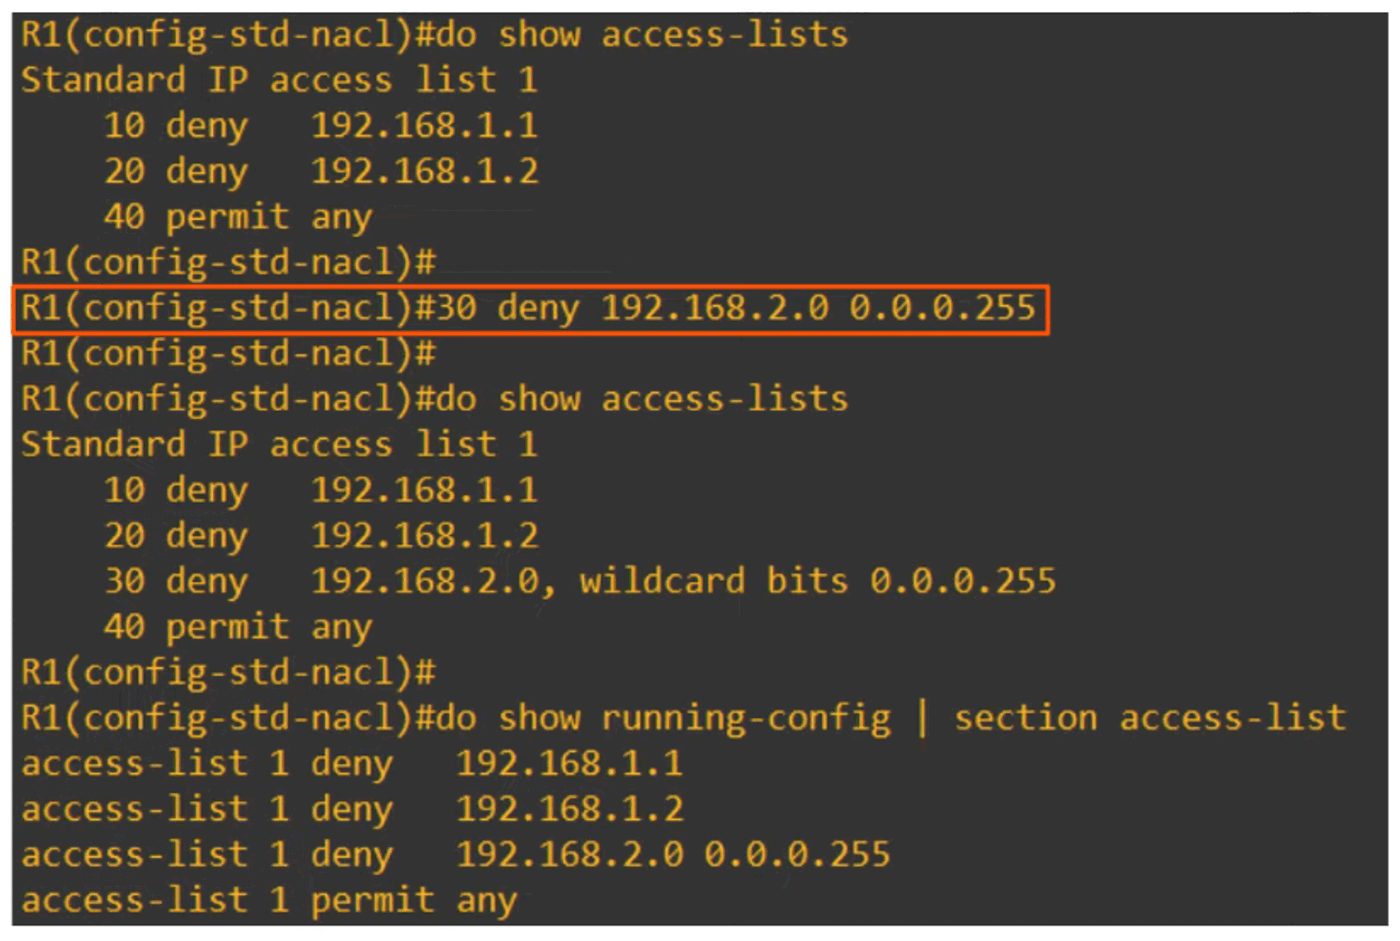
\includegraphics[keepaspectratio,alt={image}]{images/36-extended-access-control-lists/img-007.png}}
\end{figure}

RESEQUENCING ACLs

\begin{itemize}
\tightlist
\item
  There is a \emph{resequencing} function that helps edit ACLs
\item
  The command is
  \passthrough{\lstinline!R1(config)\#ip access-list resequence *acl-id starting-seq-num increment*!}
\end{itemize}

\begin{figure}
\centering
\pandocbounded{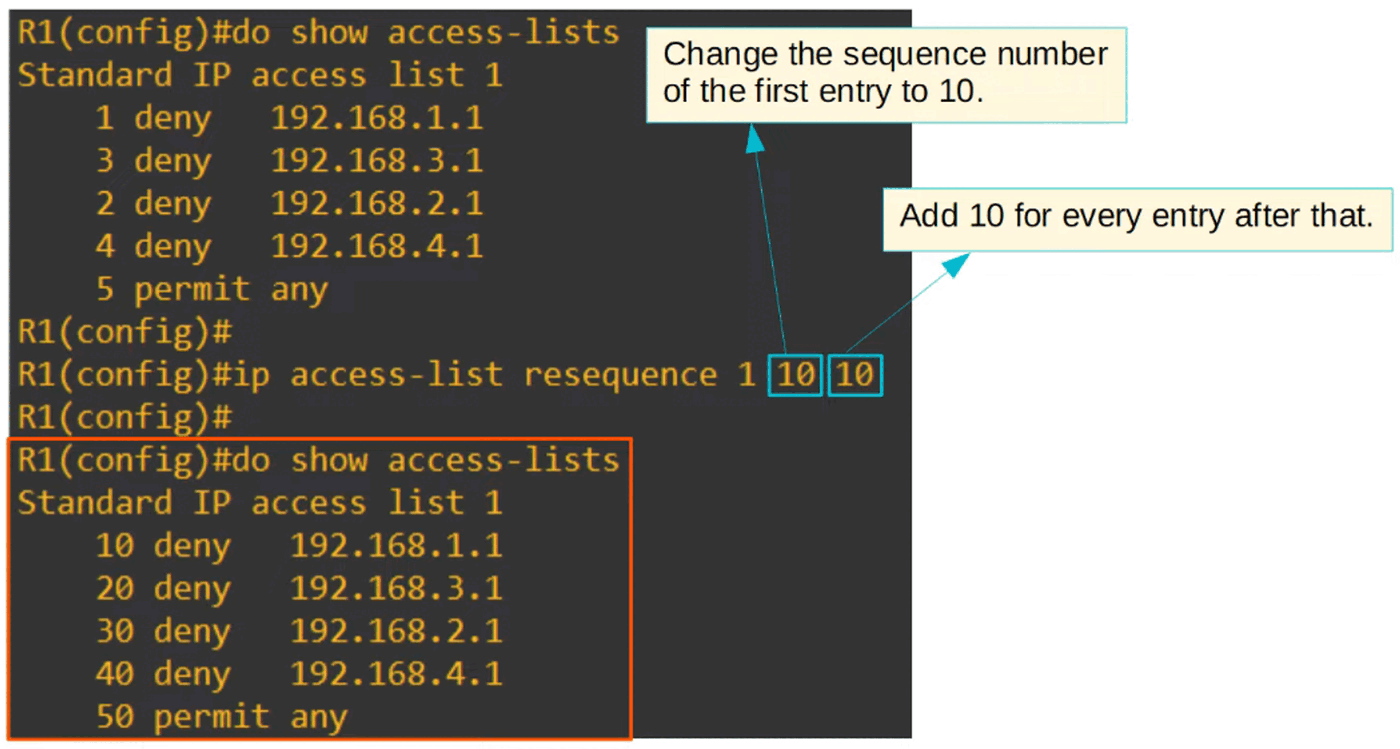
\includegraphics[keepaspectratio,alt={image}]{images/36-extended-access-control-lists/img-008.png}}
\end{figure}

EXTENDED NUMBERS AND NAMED ACLs

\begin{itemize}
\tightlist
\item
  EXTENDED ACLs function mostly the same as STANDARD ACLs
\item
  They can be NUMBERED or NAMED, just like STANDARD ACLs

  \begin{itemize}
  \tightlist
  \item
    NUMBERED ACLs use the following ranges: \textbf{100 - 199, 2000 -
    2699}
  \end{itemize}
\item
  Processed from TOP to BOTTOM, just like STANDARD ACLs
\item
  However, they can match traffic based on MORE PARAMETERS, so they are
  more PRECISE (and more complex) than STANDARD ACLs
\item
  We will focus on matching based on these main parameters:

  \begin{itemize}
  \tightlist
  \item
    \textbf{LAYER 4 protocol / port}
  \item
    \textbf{Source Address}
  \item
    D\textbf{estination Address}
  \end{itemize}
\end{itemize}

\section{Extended Numbered ACL}\label{extended-numbered-acl}

\begin{tipbox}

\passthrough{\lstinline!R1(config)\# access-list *number* [permit | deny] *protocol src-ip dest-ip*!}

\end{tipbox}

\section{Extended Named ACL}\label{extended-named-acl}

\begin{tipbox}

\passthrough{\lstinline!R1(config)\# ip access-list extended \{name | number\}!}

\end{tipbox}

\begin{tipbox}

\passthrough{\lstinline!R1(config-ext-nacl)\# \{seq-num\} \{permit | deny\} *protocol src-ip dest-ip*!}

\end{tipbox}

\section{Matching the Protocol}\label{matching-the-protocol}

\begin{figure}
\centering
\pandocbounded{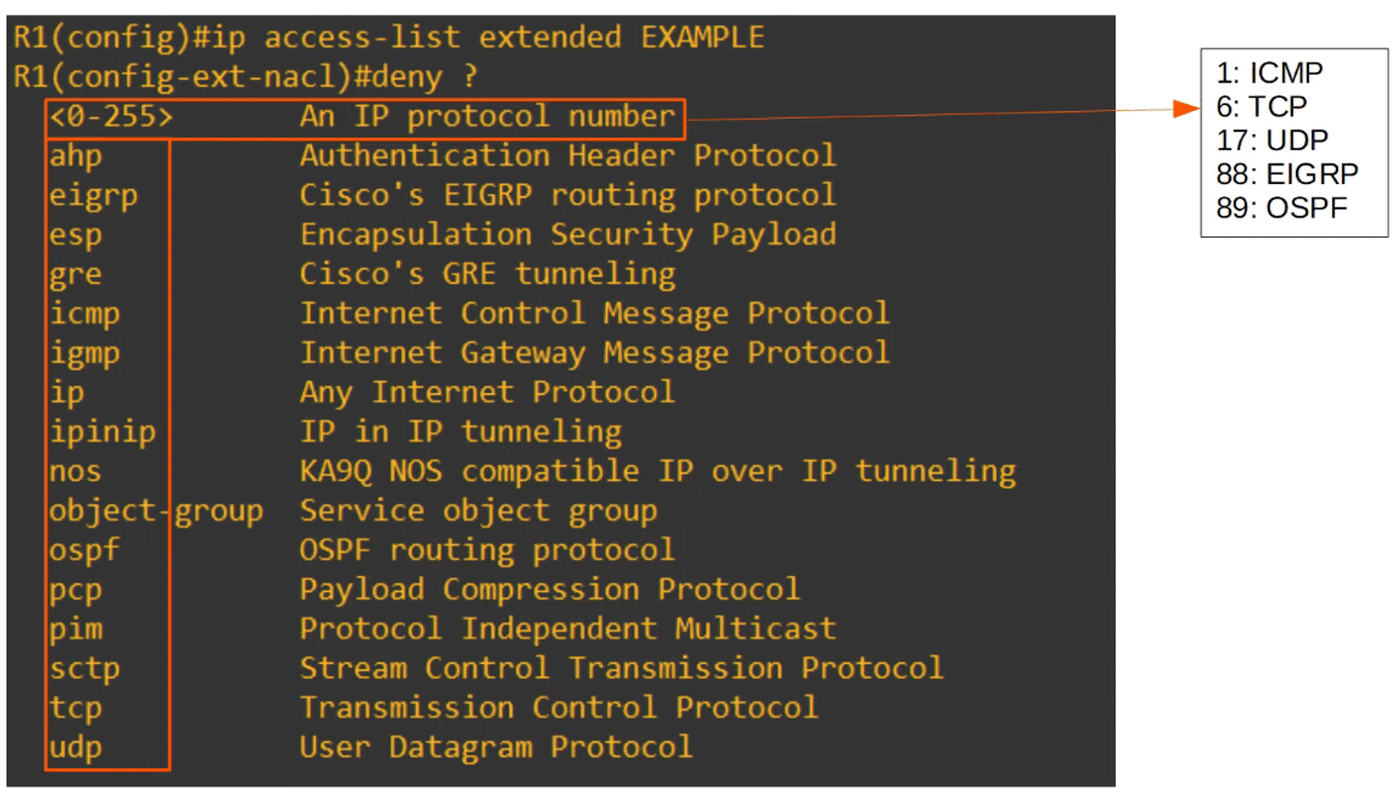
\includegraphics[keepaspectratio,alt={image}]{images/36-extended-access-control-lists/img-009.png}}
\end{figure}

IP Protocol Number is the number used in the IPv4 Header Protocol field

Examples: (1) ICMP, (6) TCP, (17) UDP, (88) EIGRP, (89) OSPF

\section{Matching the Source / Destination IP
Address}\label{matching-the-source-destination-ip-address}

\begin{figure}
\centering
\pandocbounded{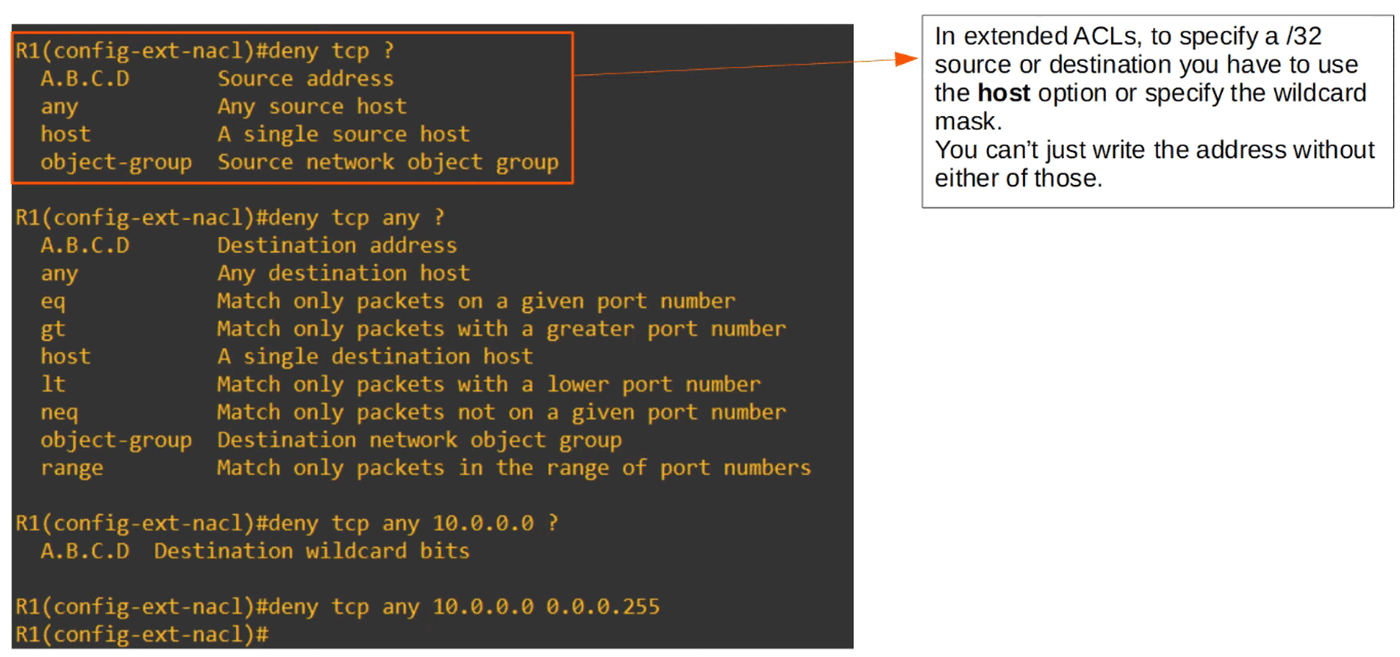
\includegraphics[keepaspectratio,alt={image}]{images/36-extended-access-control-lists/img-010.png}}
\end{figure}

This command:

\begin{tipbox}

\passthrough{\lstinline!R1(config-ext-nacl)\#deny tcp any 10.0.0.0 0.0.0.255!}

\end{tipbox}

Deny ALL PACKETS that encapsulate a TCP segment from ANY source to
DESTINATION 10.0.0.0/24

\section{Practice Questions}\label{practice-questions}

\begin{enumerate}
\def\labelenumi{\arabic{enumi})}
\tightlist
\item
  ALLOW ALL TRAFFIC
\end{enumerate}

\passthrough{\lstinline!R1(config-ext-nacl)\# permit ip any any!} (ip is
used for ``all protocols'')

\begin{enumerate}
\def\labelenumi{\arabic{enumi})}
\setcounter{enumi}{1}
\tightlist
\item
  PREVENT 10.0.0.0/16 from SENDING UDP traffic to 192.168.1.1/32
\end{enumerate}

\passthrough{\lstinline!R1(config-ext-nacl)\# deny udp 10.0.0.0 0.0.255.255 host 192.168.1.1!}

\begin{enumerate}
\def\labelenumi{\arabic{enumi})}
\setcounter{enumi}{2}
\tightlist
\item
  PREVENT 172.16.1.1/32 from pinging hosts in 192.168.0.0/24
\end{enumerate}

\passthrough{\lstinline!R1(config-ext-nacl)\# deny icmp host 172.16.1.1 192.168.0.0 0.0.0.255!}

\section{Matching the TCP / UDP Port
Numbers}\label{matching-the-tcp-udp-port-numbers}

\begin{itemize}
\tightlist
\item
  When matching TCP / UDP, you can optionally specify the SOURCE and/or
  DESTINATION PORT NUMBERS to match
\end{itemize}

\begin{figure}
\centering
\pandocbounded{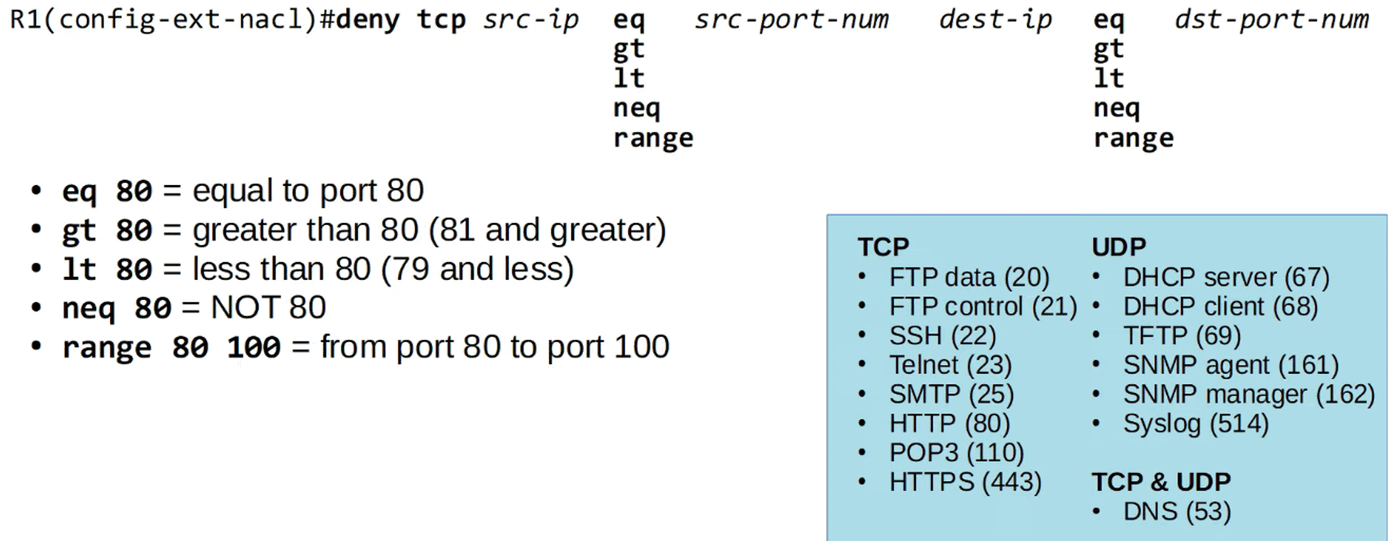
\includegraphics[keepaspectratio,alt={image}]{images/36-extended-access-control-lists/img-011.png}}
\end{figure}

eq = equal than

gt = greater than

lt = less than

neq = not equal to

range = range of ports

You can use either the PORT NUMBER or the specific TYPE (that has a
KNOWN PORT NUMBER)

\begin{figure}
\centering
\pandocbounded{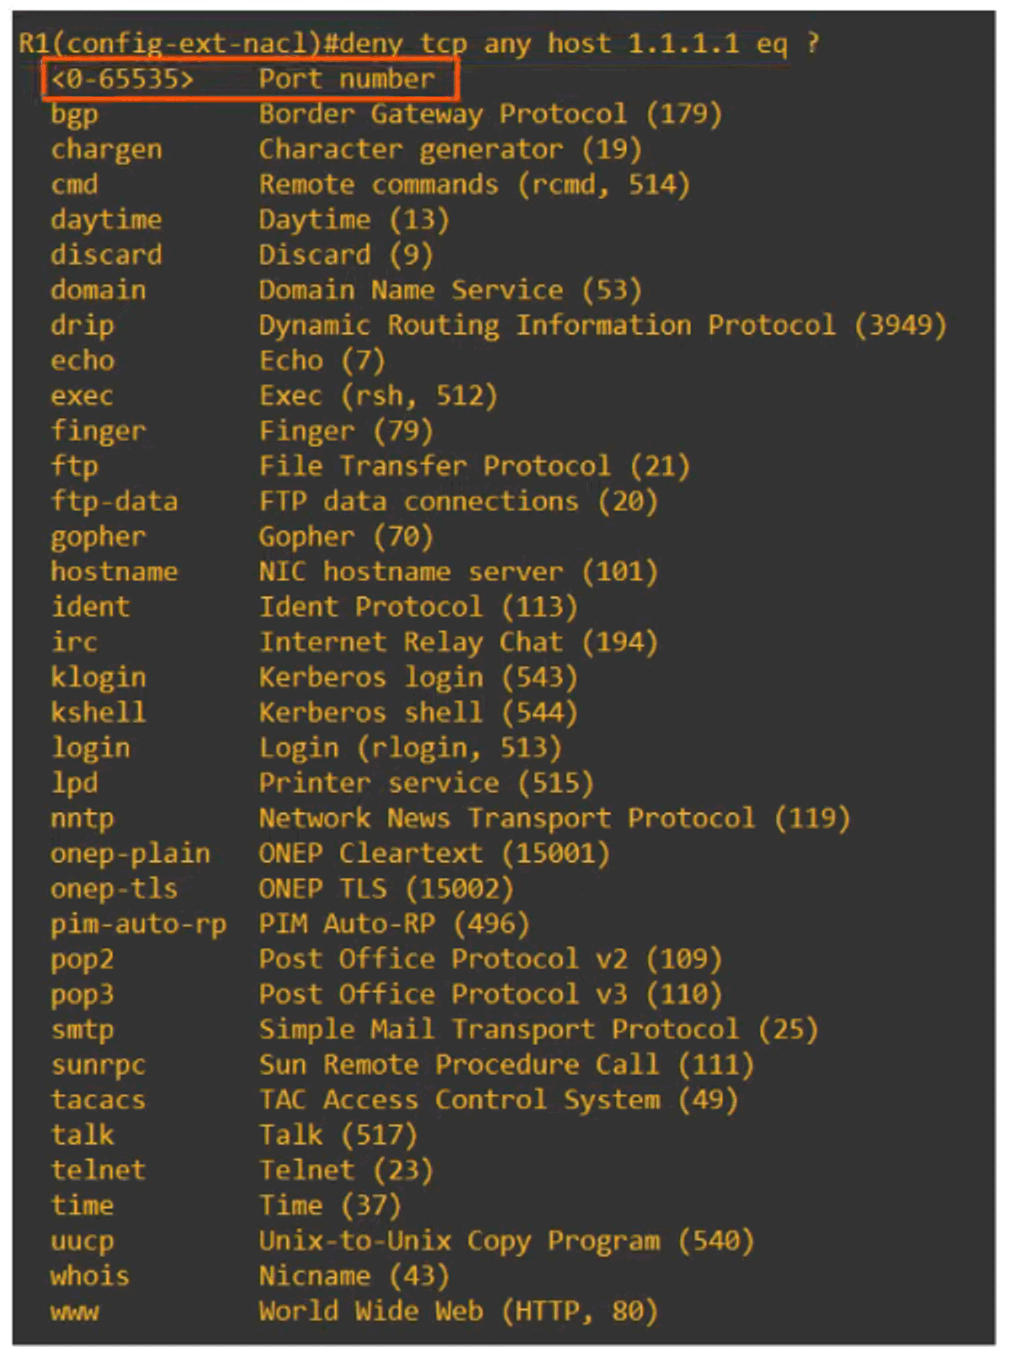
\includegraphics[keepaspectratio,alt={image}]{images/36-extended-access-control-lists/img-012.png}}
\end{figure}

\begin{figure}
\centering
\pandocbounded{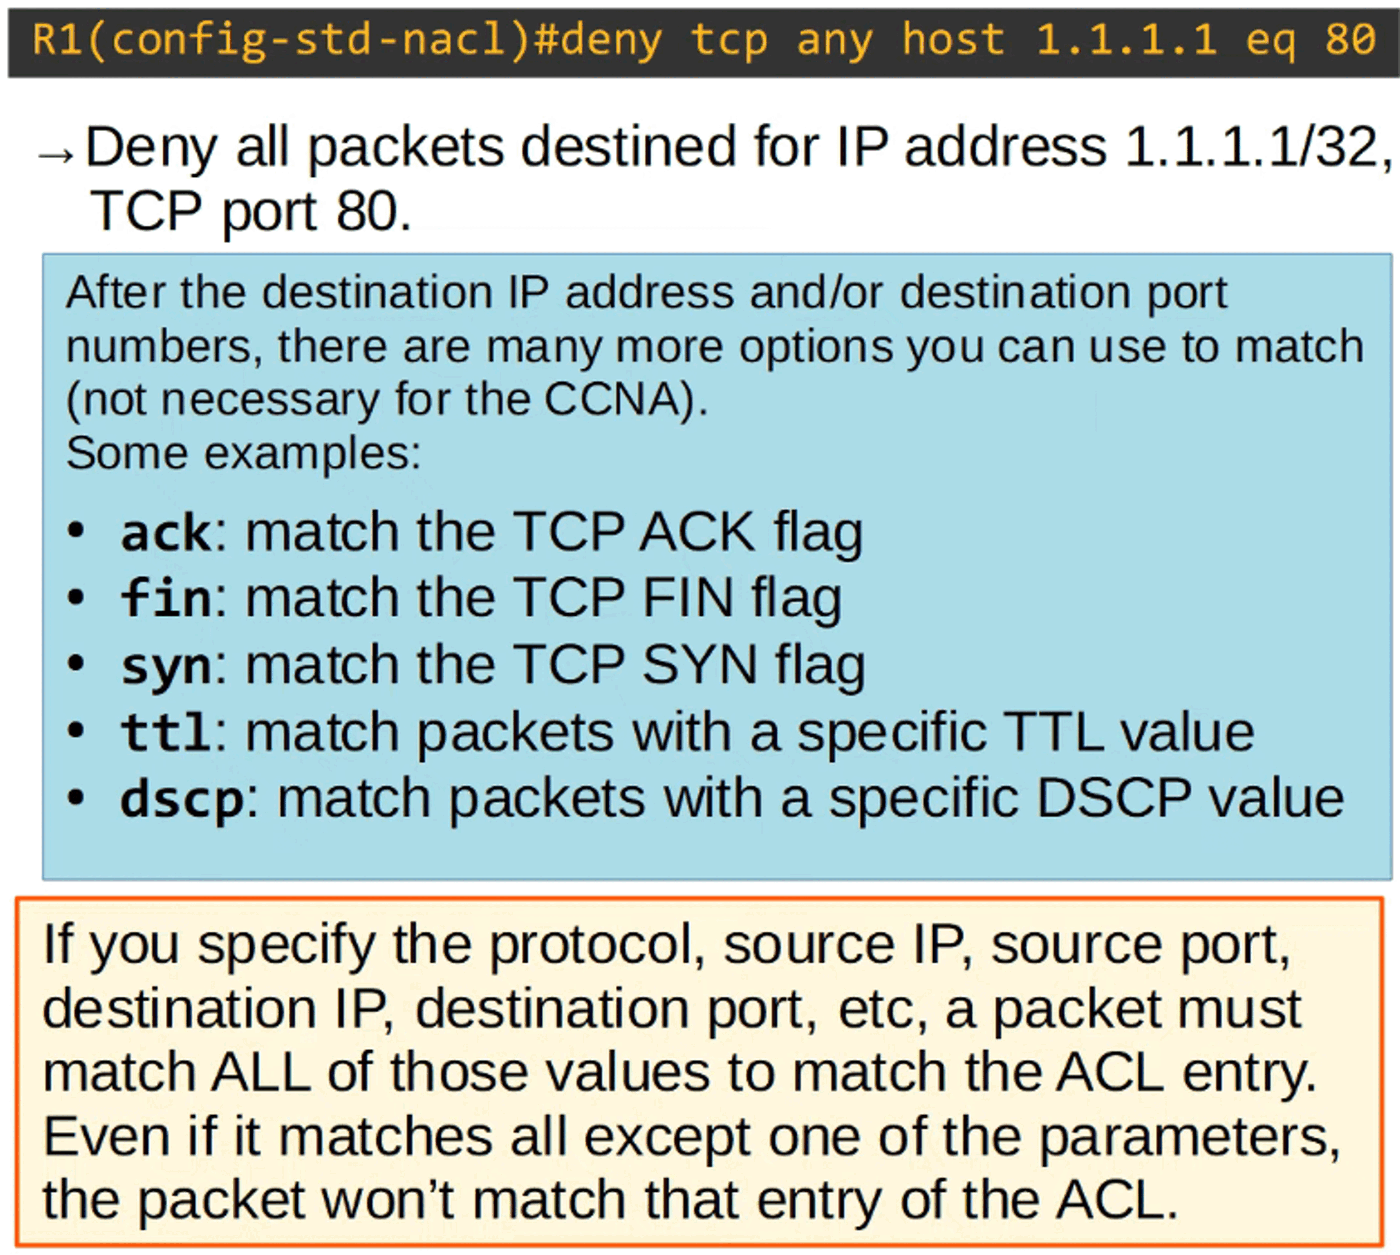
\includegraphics[keepaspectratio,alt={image}]{images/36-extended-access-control-lists/img-013.png}}
\end{figure}

\section{Practice Questions 2}\label{practice-questions-2}

\begin{enumerate}
\def\labelenumi{\arabic{enumi})}
\tightlist
\item
  ALLOW TRAFFIC from 10.0.0.0/16 to access the server at 2.2.2.2/32
  using HTTPS
\end{enumerate}

\passthrough{\lstinline!R1(config-ext-nacl)\# permit tcp 10.0.0.0 0.0.255.255 host 2.2.2.2 eq 443!}

\begin{enumerate}
\def\labelenumi{\arabic{enumi})}
\setcounter{enumi}{1}
\tightlist
\item
  PREVENT ALL HOSTS using SOURCE UDP Port Numbers from 20000 to 30000
  from accessing the server at 3.3.3.3/32
\end{enumerate}

\passthrough{\lstinline!R1(config-ext-nacl)\# deny udp any range 20000 30000 host 3.3.3.3!}

\begin{enumerate}
\def\labelenumi{\arabic{enumi})}
\setcounter{enumi}{2}
\tightlist
\item
  ALLOW HOSTS in 172.16.1.0/24 using a TCP SOURCE Port greater than 9999
  to access ALL TCP ports on server 4.4.4.4/32 EXCEPT port 23
\end{enumerate}

\passthrough{\lstinline!R1(config-ext-nacl)\# permit tcp 172.16.1.0 0.0.0.255 gt 9999 host 4.4.4.4 neq 23!}

\section{Example Network}\label{example-network}

\begin{figure}
\centering
\pandocbounded{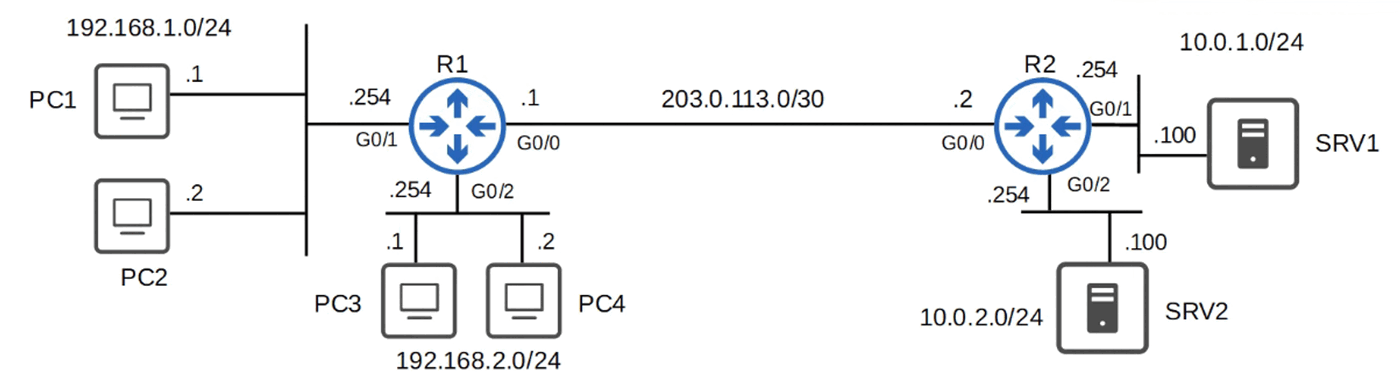
\includegraphics[keepaspectratio,alt={image}]{images/36-extended-access-control-lists/img-014.png}}
\end{figure}

\begin{figure}
\centering
\pandocbounded{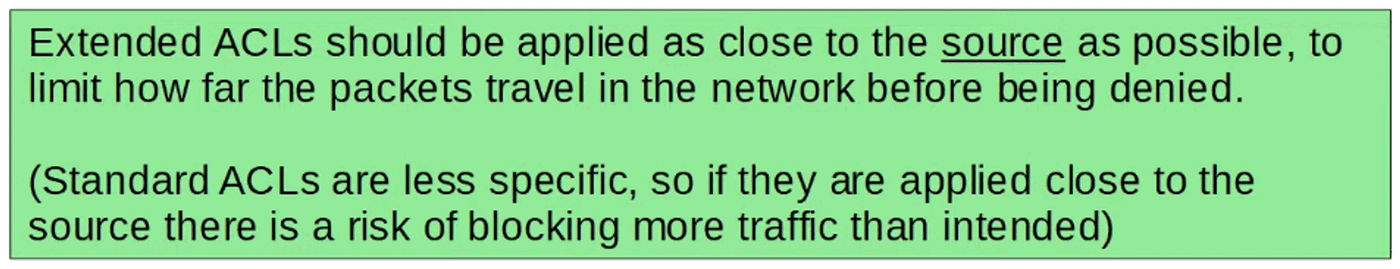
\includegraphics[keepaspectratio,alt={image}]{images/36-extended-access-control-lists/img-015.png}}
\end{figure}

\section{Requirements}\label{requirements}

\begin{itemize}
\tightlist
\item
  Hosts in 192.168.1.0/24 can't use HTTPS to access SRV1
\item
  Hosts in 192.168.2.0/24 can't access 10.0.2.0/24
\item
  NONE of the hosts in 192.168.1.0/24 or 192.168.2.0/24 can ping
  10.0.1.0/24 OR 10.0.2.0/24
\end{itemize}

EXTENDED ACL \#1 (Applied at R1 G0/1 INBOUND interface)

\passthrough{\lstinline!R1(config)\# ip access-list extended HTTP\_SRV1!}
\passthrough{\lstinline!R1(config-ext-nacl)\# deny tcp 192.168.1.0 0.0.0.255 host 10.0.1.100 eq 443!}

\passthrough{\lstinline!R1(config-ext-nacl)\# permit ip any any!}

\passthrough{\lstinline!R1(config-ext-nacl)\# int g0/1!}

\passthrough{\lstinline!R1(config-if)\# ip access-group HTTP\_SRV1 in!}

EXTENDED ACL \#2 (APPLIED at R1 G0/2 INBOUND interface)

\passthrough{\lstinline!R1(config)\# ip access-list extended BLOCK\_10.0.2.0!}

\passthrough{\lstinline!R1(config-ext-nacl)\# deny ip 192.168.2.0 0.0.0.255 10.0.2.0 0.0.0.255!}

\passthrough{\lstinline!R1(config-ext-nacl)\# permit ip any any!}

\passthrough{\lstinline!R1(config-ext-nacl)\# int g0/2!}

\passthrough{\lstinline!R1(config-if)\# ip access-group BLOCK\_10.0.2.0 in!}

EXTENDED ACL \#3 (APPLIED at R1 g0/0 OUTBOUND interface)

\passthrough{\lstinline!R1(config)\# ip access-list extended BLOCK\_ICMP!}

\passthrough{\lstinline!R1(config-ext-nacl)\# deny icmp 192.168.1.0 0.0.0.255 10.0.1.0 0.0.0.255!}

\passthrough{\lstinline!R1(config-ext-nacl)\# deny icmp 192.168.1.0 0.0.0.255 10.0.2.0 0.0.0.255!}

\passthrough{\lstinline!R1(config-ext-nacl)\# deny icmp 192.168.2.0 0.0.0.255 10.0.1.0 0.0.0.255!}

\passthrough{\lstinline!R1(config-ext-nacl)\# permit ip any any!}

\passthrough{\lstinline!R1(config-ext-nacl)\# int g0/0!}

\passthrough{\lstinline!R1(config-if)\# ip access-group BLOCK\_ICMP out!}

What the EXTENDED ACLs look like

\begin{figure}
\centering
\pandocbounded{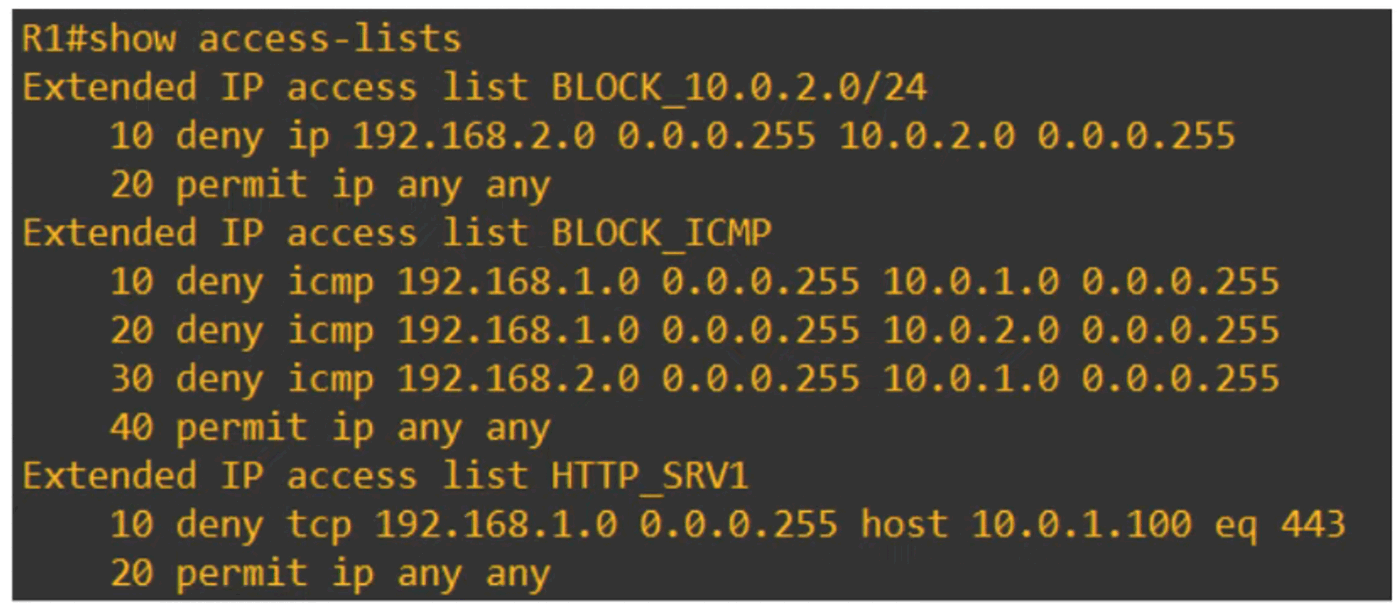
\includegraphics[keepaspectratio,alt={image}]{images/36-extended-access-control-lists/img-016.png}}
\end{figure}

HOW TO SEE WHICH EXTENDED ACL's ARE APPLIED TO AN INTERFACE

\begin{figure}
\centering
\pandocbounded{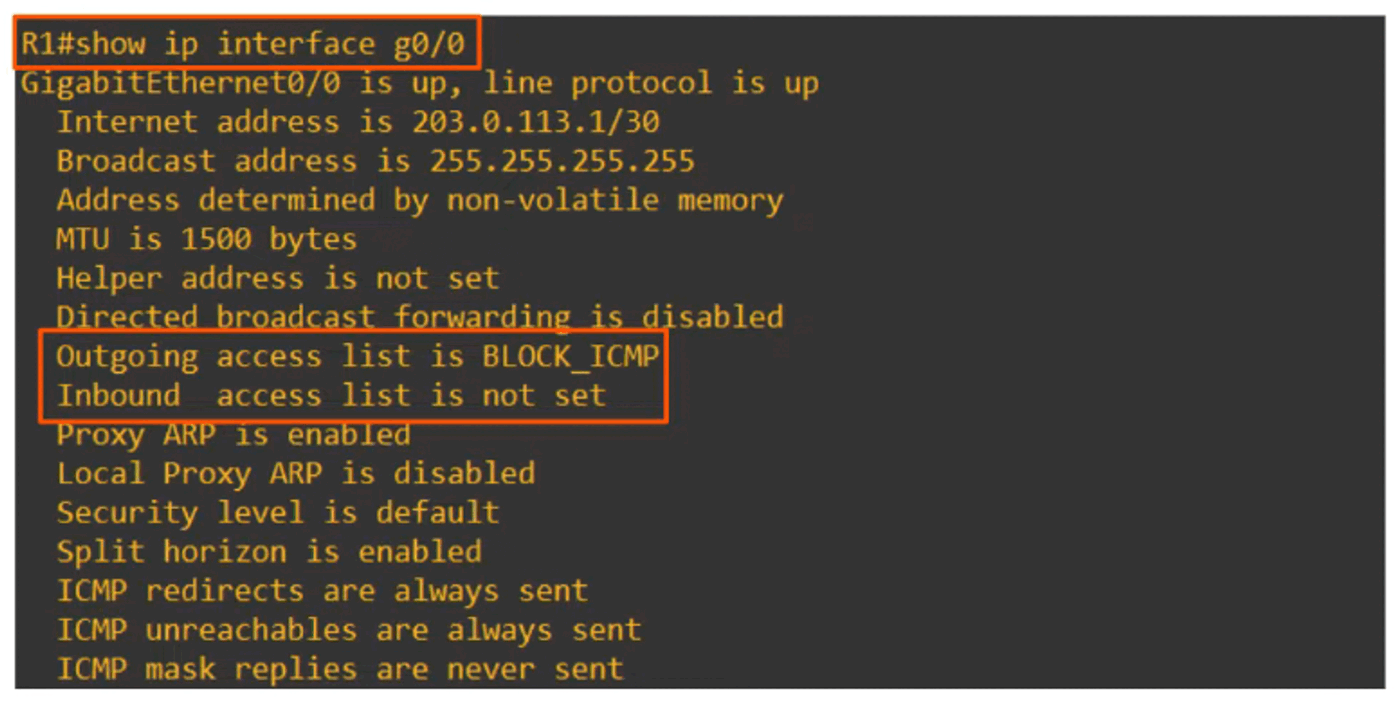
\includegraphics[keepaspectratio,alt={image}]{images/36-extended-access-control-lists/img-017.png}}
\end{figure}
